\documentclass[11pt]{article}

%-----------------------------------------------------------%
%-------------TEST POUR LA FICHE DE SYNTHESE----------------%
%-----------------------------------------------------------%

\usepackage{geometry}
\usepackage{lipsum}
\usepackage{xcolor}
\usepackage{graphicx}

\pagestyle{empty}
\geometry{a4paper}
\geometry{top=0.5cm, bottom=2cm, left=1cm, right=1cm}

\begin{document}
\parindent=0pt

%Debut de l'entete------------------------------------------%
%------------------Les logos--------------------------------%
\begin{minipage}{0.55\linewidth}
    \begin{flushleft}
    
\includegraphics[scale=0.28]{ESRF_logo.png}
    \end{flushleft}
\end{minipage}
\hfill
\begin{minipage}{0.40\linewidth}
    \begin{center}
    
\includegraphics[scale=0.28]{logo-lille1-2014.png}
    \end{center}
\end{minipage}

\vspace{0.2cm}
\hrulefill
\vspace{0.2cm}

%------------------Bloc de gauche---------------------------%
\begin{minipage}{0.25\linewidth}
    \begin{center}
    \textbf{Guillaume Bonamis}\\
    \textbf{Master 1 Physique}\\ %en francais ou en anglais ???
    \textbf{2014-2015}
    \end{center}
\end{minipage}
%------------------Bloc du centre---------------------------%
\hfill
\begin{minipage}{0.30\linewidth}
    \begin{center} 
    \textbf{Universit\'e Lille 1}\\
    \textbf{UFR de Physique}\\

    Tutor: Emeline Dudognon
    \end{center}
\end{minipage}
%------------------Bloc de droite---------------------------%
\hfill
\begin{minipage}{0.30\linewidth}
    \begin{center}
    \textbf{ESRF}\\
    \textbf{Data Analysis Unit}\\

    Supervisor: J\'er\^ome Kiffer
    \end{center}
\end{minipage}
%Fin de l'entete--------------------------------------------%


%Intitule du stage------------------------------------------%
\begin{center}
    \fbox{\begin{minipage}{\linewidth}
    \begin{center}\bfseries\Huge 
        Intitul\'e du stage de Master 1
    \end{center}
    \end{minipage}}
\end{center}
%-----------------------------------------------------------%


%Introduction du sujet--------------------------------------%
\begin{center}%Il faudra surement faire plus court, plus rentre dedans
\fbox{\begin{minipage}{\linewidth}
    \textbf{Abstract}: 
    A new implementation of a method for the optimised alignment of 
    three-dimensional models is presented. 
    It uses the superimposition of centers of mass and principal axis of 
    inertia of the models and measures the quality of the alignment with a 
    metric called Normalized Spatial Discrepancy (NSD). 
    This implementation has been used to create a program called SuPyComb. 
    It allows the comparison of the models obtained from the treatment of 
    scattering curves from Small Angles Scattering (SAS) experiments.
\end{minipage}}
\end{center}
%-----------------------------------------------------------%


%Essai bloc texte a gauche, image a droite------------------%
\begin{minipage}{0.55\linewidth}
    A new implementation of a method for the optimised alignment of 
    three-dimensional models is presented. 
    It uses the superimposition of centers of mass and principal axis of 
    inertia of the models and measures the quality of the alignment with a 
    metric called Normalized Spatial Discrepancy (NSD). 
    This implementation has been used to create a program called SuPyComb. 
    It allows the comparison of the models obtained from the treatment of 
    scattering curves from Small Angles Scattering (SAS) experiments.
    A new implementation of a method for the optimised alignment of 
    three-dimensional models is presented. 
    A new implementation of a method for the optimised alignment of 
    three-dimensional models is presented. 
\end{minipage} \hfill
\begin{minipage}{0.4\linewidth}
    \begin{flushleft}
    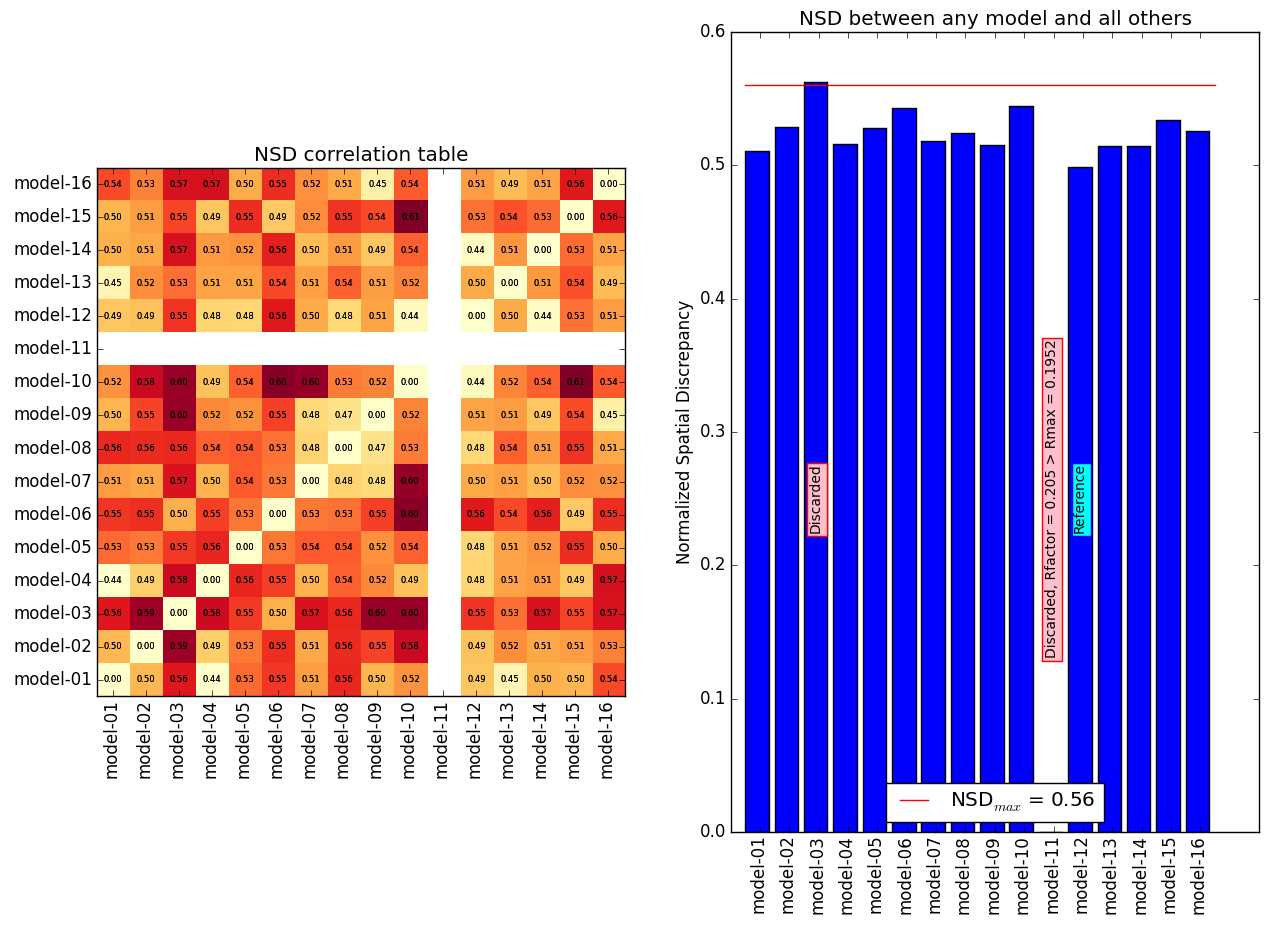
\includegraphics[scale=0.4]{nsd.png}
    \end{flushleft}
\end{minipage}
%-----------------------------------------------------------%


%Notes de fin-----------------------------------------------%
\begin{center}
\fbox{\begin{minipage}{\linewidth}
\begin{minipage}{0.45\linewidth}
    Une place de pr\^ete pour plus tard
\end{minipage}
\hfill
\begin{minipage}{0.45\linewidth}
    Et une autre au cas o\`u
\end{minipage}

\begin{minipage}{0.95\linewidth}
    \textbf{Keywords}: 
    le premier mot, le deuxi\`eme, et le troisi\`eme
\end{minipage}
\end{minipage}
}
\end{center}
%-----------------------------------------------------------%
\end{document}
